\documentclass[11pt]{article}

\usepackage[letterpaper,margin=0.80in]{geometry}
\usepackage{amsmath,amssymb,mathtools,bm}
\usepackage{amsthm}
\usepackage{microtype}
\usepackage{setspace}
\usepackage{caption}
\usepackage{balance}
\usepackage{titlesec}
\usepackage{enumitem}
\usepackage{booktabs}
\usepackage{array}
\usepackage{hyperref}
\usepackage{xcolor}
\usepackage{graphicx}
\usepackage{tikz}
\usetikzlibrary{arrows.meta,calc,positioning,fit,backgrounds}

\setstretch{1.10}
\setlength{\parskip}{0.35em}
\setlength{\parindent}{1.25em}
\setlength{\columnsep}{0.28in}
\raggedbottom
\setlength{\emergencystretch}{2em}
\captionsetup{font=small,labelfont=bf}

% Keep section headings ragged-right and strongly discourage word hyphenation.
\titleformat{\section}
  {\large\bfseries\raggedright\hyphenpenalty=10000\exhyphenpenalty=10000}
  {\thesection}{0.55em}{}
\titleformat{\subsection}
  {\normalsize\bfseries\raggedright\hyphenpenalty=10000\exhyphenpenalty=10000}
  {\thesubsection}{0.50em}{}
\titlespacing*{\section}{0pt}{1.15em}{0.45em}
\titlespacing*{\subsection}{0pt}{0.90em}{0.35em}

\hypersetup{
  hidelinks,
  pdftitle={Spacetime as Source-Local Rollout and the Conditional Emergence of Three-Dimensional Effective Geometry in The Emergent Frame},
  pdfauthor={Xiaodan Wu},
  pdfinfo={ORCID={0009-0005-5892-0293}, Version={3.12}, DOI={10.5281/zenodo.22776137}}
}

\newtheorem{proposition}{Proposition}
\newtheorem{lemma}{Lemma}
\newtheorem{remark}{Remark}
\newtheorem{assumption}{Working Postulate}
\newtheorem{definition}{Definition}
\renewcommand{\qedsymbol}{}

\newcommand{\TEF}{\mathrm{TEF}}
\newcommand{\dd}{\mathrm{d}}
\newcommand{\Z}{\mathbb{Z}}
\newcommand{\R}{\mathbb{R}}
\newcommand{\SO}{\mathrm{SO}}
\newcommand{\U}{\mathrm{U}}
\newcommand{\cX}{\mathcal{X}}
\newcommand{\cU}{\mathcal{U}}
\newcommand{\cF}{\mathcal{F}}
\newcommand{\cV}{\mathcal{V}}
\newcommand{\cE}{\mathcal{E}}
\newcommand{\cL}{\mathcal{L}}
\newcommand{\cK}{\mathcal{K}}
\newcommand{\cG}{\mathcal{G}}
\newcommand{\conceptbox}[1]{\begin{center}\fbox{\parbox{0.91\columnwidth}{\centering #1}}\end{center}}

\title{\bfseries Spacetime as Source-Local Rollout and the Conditional Emergence of Three-Dimensional Effective Geometry in The Emergent Frame}

\author{\small Xiaodan Wu\textsuperscript{1,*}\\[-0.10em]
\footnotesize \textsuperscript{1}Independent Researcher\textsuperscript{\(\dagger\)}}
\date{\footnotesize September 2026 \quad Version 3.12}

\begin{document}
\twocolumn[
\begin{@twocolumnfalse}
\maketitle
\vspace{-0.85em}
\begingroup
\normalsize
\setstretch{1.10}
\begin{center}
\textbf{Abstract}
\end{center}
\noindent
The Emergent Frame (TEF) treats spacetime not as a pre-existing common background but as relational structure continuously realized by closed matter through spacetime rollout. This paper gives a conditional mathematical realization of that view using a source-local ensemble of helical rollout trajectories whose transverse relational organization is represented by a weighted two-dimensional cell complex. In the homogeneous transported-complex ground state, intrinsic untwisting yields a product of spatial rollout depth and the transverse complex, producing cubic volume growth with \(d_f=3\). Under explicit long-scale graph-analytic conditions, the same construction gives normal diffusion with \(d_w=2\) and a bulk static Green scale \(G(x,y)\asymp d(x,y)^{-1}\). The familiar \(1/r\) behavior therefore arises as a forward consequence of the candidate rollout geometry, while hydrogenic \(1/n^2\) gross scaling remains only a low-energy consistency check.

The construction is deliberately conditional: the two-dimensional quadratic-growth organization of the full rollout ensemble is a TEF structural postulate, not a result forced by one isolated helix. The same ontology also suggests a source-local cosmogenesis---a continuous ``TEF Big Bang'' in which each closed matter source realizes its own rollout universe. That interpretation is not yet a quantitative cosmological model; a shared effective world must ultimately emerge from compatibility among many source-local rollout structures.

\endgroup
\vspace{1.15em}
\end{@twocolumnfalse}
]
\begingroup
\renewcommand{\thefootnote}{\fnsymbol{footnote}}
\footnotetext[1]{\href{mailto:xiaodan@theemergentframe.org}{xiaodan@theemergentframe.org}}
\footnotetext[2]{\href{https://theemergentframe.org}{https://theemergentframe.org}; ORCID: \href{https://orcid.org/0009-0005-5892-0293}{0009-0005-5892-0293}; DOI: \href{https://doi.org/10.5281/zenodo.22776137}{10.5281/zenodo.22776137}.}
\endgroup


\section{Introduction}

The conventional geometric language of physics normally begins with a spacetime manifold or another global kinematic arena on which matter and fields are defined. TEF reverses that order. Its working ontology is that closed matter is a source of spacetime rollout: spatial relations are continuously realized by the source rather than presupposed as a common background \cite{WuFramework2026}.

Earlier TEF work introduced a local helical rollout ansatz and explored cross-sector correspondences involving a primitive length scale and a frozen dimensionless helix parameter \(q\) \cite{WuHelix2026,WuAlpha2026}. Those numerical correspondences are not the subject of the present paper. The present problem is more structural:

\conceptbox{Can a source-local helical rollout ontology support
\(d_f=3\), \(d_w=2\), and \(G(r)\propto 1/r\)?}

The question should not be asked by staring at one isolated helical curve. A physical rollout source is taken here to generate an ensemble of rollout trajectories. The ensemble, its adjacency relations, and the way it is transported from one spatial rollout depth to another are the relevant microscopic objects.

The paper has three aims: to state the TEF spacetime postulates used here; to construct and analyze a transported source-local relational complex; and to separate the resulting mathematical claims from broader interpretations involving transverse transport, excitations, and source-local cosmogenesis.

The contribution is deliberately narrow. TEF does not claim priority for emergent spacetime, relational geometry, spectral dimension, or coherence-based gauge structure as general ideas. The specific construction developed here combines a source-local helical rollout ontology with an explicit transported relational complex and derives, conditionally, cubic volume growth, normal long-scale diffusion, and a \(1/r\)-type bulk Green scale.

\subsection{Compatibility rather than ontological equivalence}

A viable TEF theory must reproduce established observations in tested regimes without necessarily sharing the ontology of the effective theories that describe them. The intended logic is
\conceptbox{TEF postulates $\longrightarrow$ emergent effective structure $\longrightarrow$ observational compatibility}
Three-dimensional growth, normal propagation, Abelian transverse transport, and \(1/r\) static response are therefore consistency targets, not primitive assumptions about a common background spacetime.


\section{Related work and novelty boundary}

Several research programs share parts of this motivation. The comparisons below locate the TEF claim without treating nearby work as empirical support.

\paragraph{Emergent locality from microscopic relational structure.}
Quantum Graphity is direct prior art for emergent locality from microscopic relational adjacency: dynamical graphs can develop an ordered, low-dimensional local phase, with an emergent \(\U(1)\) sector also discussed \cite{Konopka2008}. TEF uses a different microscopic ontology and construction.

\paragraph{Pre-geometric and condensate approaches to spacetime emergence.}
Group Field Theory (GFT) likewise treats continuum spacetime as emergent from more microscopic, non-continuum degrees of freedom, often through collective or condensate descriptions \cite{Oriti2007}. TEF instead takes closed matter as a source of local spacetime rollout and uses a helical rollout ensemble as its working microscopic picture.

\paragraph{Random-walk and spectral probes of effective dimension.}
Random walks and spectral dimension are standard probes of effective dimensionality in discrete spacetime models; causal-set work provides one example \cite{EichhornMizera2014}. Here the corresponding heat-kernel language accompanies an explicit volume-growth theorem for a transported source-local complex.

\paragraph{Relational coherence, transport, and gauge structure.}
Recent preprints also explore pre-geometric frameworks built from coherent relational transport, holonomy, and compact coherence structure \cite{Arneth2026PreEinsteinian,Arneth2026Twisted}. They are cited here as nearby conceptual work. The specific construction developed in this paper is the source-local helical rollout ensemble together with the transported relational complex analyzed below.

Accordingly, the narrower novelty claim is

\conceptbox{source-local helical rollout ontology
\(+\) transported transverse relational complex
\(+\) conditional \(d_f=3\), \(d_w=2\), \(G(r)\asymp r^{-1}\) derivation}

The source-local interpretation further requires a future multi-source compatibility rule; no quantitative composition theory is derived here.

\section{Working spacetime postulates}

The present construction uses four TEF postulates. They are not claimed here to be final axioms of nature. They are hypotheses whose consequences can be checked against mathematics and observation.

\begin{assumption}[Closed matter is a source of spacetime rollout]
A stable closed matter structure \(S\) continuously realizes a source-local rollout structure
\[
S \longrightarrow \cU_S .
\]
The structure \(\cU_S\) is not interpreted as a pre-existing public background into which the source is inserted.
\end{assumption}

\begin{assumption}[The source generates an ensemble of helical rollout trajectories]
The microscopic rollout object associated with \(S\) is a family
\[
\Gamma_S=\{\gamma_\alpha\}_{\alpha\in A_S},
\]
not a single isolated curve. Each regular local trajectory has a longitudinal tangent and an oriented two-dimensional transverse frame.
\end{assumption}

\begin{assumption}[Homogeneous ground-state rollout is regular and screw-isometric]
In a homogeneous, defect-free sector, spatial rollout depth is advanced by a regular one-parameter screw-isometric continuation. Its action on the local transverse frame is orientation preserving and metric compatible.
\end{assumption}

\begin{assumption}[Excitations are collective modes of the rollout ensemble]
An excitation does not create a new independent rollout source. It is a collective configuration involving more than one rollout trajectory, with local phase coherence or phase locking among neighboring lines as a candidate microscopic mechanism. Detailed excitation dynamics are not derived in this paper.
\end{assumption}

The fourth postulate is not needed to prove the spatial growth theorem below. It is included because it constrains the physical meaning of transverse adjacency: the neighboring rollout lines must support relational coupling if collective excitations are to exist.

\section{Local helical geometry and the distinction between three structures}

A representative local helix is
\begin{equation}
\mathbf r(\varphi)
=
\bigl(R\cos\varphi,\,
R\sin\varphi,\,
qR\varphi\bigr),
\label{eq:helix}
\end{equation}
with primitive radius \(R\) and dimensionless pitch ratio \(q\). Its Frenet curvature and torsion are
\begin{equation}
\begin{aligned}
\kappa_h &= \frac{1}{R(1+q^2)},\\
\tau_h &= \frac{q}{R(1+q^2)},\\
q &= \frac{\tau_h}{\kappa_h}.
\end{aligned}
\end{equation}

At each regular point, the unit tangent is denoted \(\mathbf e_3\). An oriented orthonormal basis \((\mathbf e_1,\mathbf e_2)\) spans the transverse normal plane.

\begin{figure}[t]
\centering
\resizebox{0.98\columnwidth}{!}{
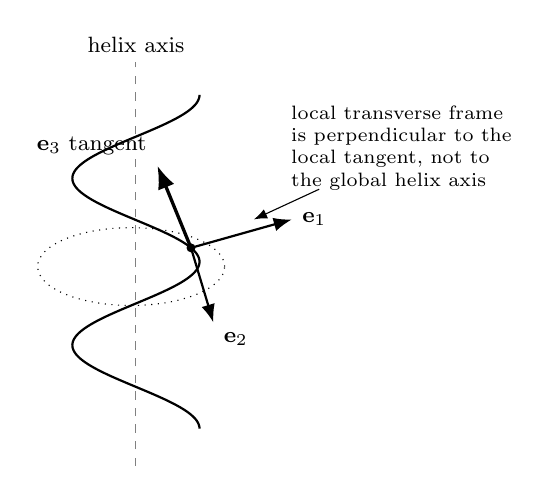
\begin{tikzpicture}[scale=0.95,>=Latex]
  % helix axis
  \draw[dashed,gray] (0,-0.5) -- (0,4.9) node[above,black,font=\footnotesize] {helix axis};
  % stylized helix
  \draw[domain=0:720,samples=220,smooth,variable=\t,thick]
    plot ({0.85*cos(\t)},{0.0062*\t});
  % point and tangent, chosen around t=390 degrees
  \coordinate (P) at ({0.85*cos(390)},{0.0062*390});
  \fill (P) circle (1.7pt);
  \draw[->,very thick] (P) -- ++(-0.45,1.10) node[above left,font=\footnotesize] {$\mathbf e_3$ tangent};
  \draw[->,thick] (P) -- ++(1.35,0.38) node[right,font=\footnotesize] {$\mathbf e_1$};
  \draw[->,thick] (P) -- ++(0.30,-1.00) node[below right,font=\footnotesize] {$\mathbf e_2$};
  \draw[dotted] ($(P)+(-0.8,-0.25)$) ellipse (1.25 and 0.52);
  \node[align=left,font=\scriptsize] at (3.55,3.75) {local transverse frame\\is perpendicular to the\\local tangent, not to\\the global helix axis};
  \draw[->,thin] (2.45,3.20) -- ($(P)+(0.84,0.38)$);
\end{tikzpicture}
}
\caption{Schematic projected local helix geometry (not metrically to scale). The longitudinal vector \(\mathbf e_3\) denotes the local tangent to the helix. The transverse frame \((\mathbf e_1,\mathbf e_2)\) is attached to that tangent; it is not defined by the global helix axis.}
\label{fig:localhelix}
\end{figure}

Five different mathematical objects must be kept separate.

\paragraph{Local normal plane of one trajectory.}
At each regular point of a single helix, the plane orthogonal to the local tangent is a two-dimensional geometric normal fiber. It is a local object attached to that trajectory.

\paragraph{Trajectory-label / transverse relational complex.}
The complex \(\cK_\perp\) introduced below represents relations among neighboring rollout trajectories in the full ensemble. It is not identified by definition with the normal plane of one helix, nor with the plane orthogonal to the global helix axis. Relating these structures is part of the TEF construction.

\paragraph{Continuous transverse-frame transport.}
A change of local transverse orthonormal frame is represented by
\[
\tau\in\SO(2).
\]
It is meaningful here to write
\[
\det \tau=1.
\]

\paragraph{Discrete cell-complex transport.}
A microscopic spatial discretization is represented by a cell-complex isomorphism
\[
T_m:\cK_m\rightarrow\cK_{m+1}.
\]
The relevant conditions are preservation of incidence, edge scale, and cell measure. A determinant is not assigned to \(T_m\) as a graph or cell map.

\paragraph{Measure transport.}
If the continuous transverse transport is metric compatible, its induced area form is preserved. In the discrete realization, the corresponding cell weights are required to be transported consistently.

Keeping these objects distinct prevents frame transport, discrete adjacency, and measure transport from being conflated.

\section{The rollout ensemble and an effective transverse relational complex}

The source-local object is the ensemble
\[
\Gamma_S=\{\gamma_\alpha\}_{\alpha\in A_S}.
\]
Ultimately, topology, adjacency, and measure on the trajectory labels \(A_S\) should be derived from relations among rollout lines. Here their homogeneous transverse organization is represented by a weighted two-dimensional cell complex
\[
\cK_\perp .
\]

\begin{assumption}[Uniform transverse relational geometry]
The reference transverse complex \(\cK_\perp\) is connected, locally finite, and equipped with edge lengths and vertex/cell weights satisfying uniform bounds
\begin{equation}
\begin{aligned}
0&<\ell_-\le \ell(e)\le \ell_+<\infty,\\
0&<m_-\le m(v)\le m_+<\infty.
\end{aligned}
\label{eq:uniformweights}
\end{equation}
Its metric-measure balls satisfy uniform quadratic growth
\begin{equation}
c_- r^2
\le
\mu_\perp(B_\perp(x,r))
\le
c_+ r^2
\label{eq:quadratic}
\end{equation}
through the homogeneous scale range of interest, with constants independent of \(x\).
\end{assumption}

The important logical point is explicit: Eq.~\eqref{eq:quadratic} is a current TEF structural hypothesis about the collective rollout ensemble. It is not derived merely from the fact that one helical trajectory possesses a formal two-dimensional normal plane.

\begin{figure}[t]
\centering
\resizebox{0.98\columnwidth}{!}{
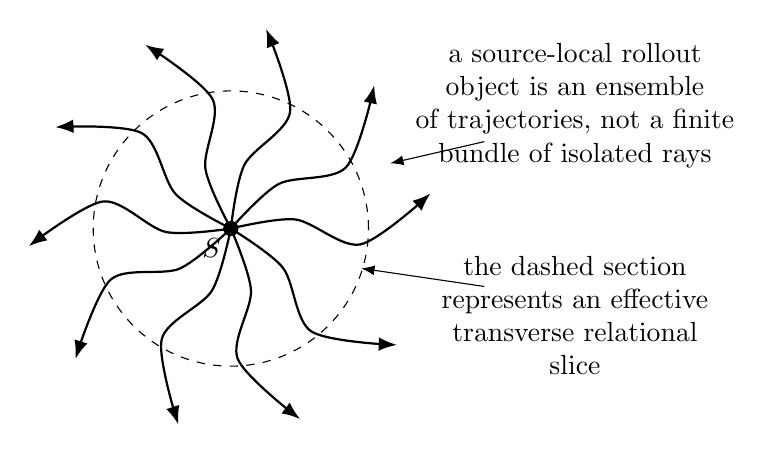
\begin{tikzpicture}[>=Latex,scale=0.92]
  \fill (0,0) circle (3pt) node[below left] {$S$};
  \foreach \ang in {0,35,70,105,140,175,210,245,280,315}{
    \draw[->,thick]
      plot[smooth] coordinates
      {(0,0)
       ({0.9*cos(\ang+8)},{0.9*sin(\ang+8)})
       ({1.8*cos(\ang-7)},{1.8*sin(\ang-7)})
       ({2.8*cos(\ang+10)},{2.8*sin(\ang+10)})};
  }
  \draw[dashed] (0,0) circle (1.9);
  \node[align=center] at (4.75,1.7) {a source-local rollout\\object is an ensemble\\of trajectories, not a finite\\bundle of isolated rays};
  \draw[->] (3.5,1.2)--(2.2,0.9);
  \node[align=center] at (4.75,-1.2) {the dashed section\\represents an effective\\transverse relational\\slice};
  \draw[->] (3.5,-0.8)--(1.8,-0.55);
\end{tikzpicture}
}
\caption{Schematic source-local rollout ensemble. The drawing is relational, not a claim that the source sits inside a pre-existing Euclidean background. The effective transverse complex is intended to represent relations among neighboring rollout trajectories at fixed spatial rollout depth.}
\label{fig:ensemble}
\end{figure}

\section{Spatial rollout depth is not physical time}

The rollout construction uses two distinct parameters.

\begin{definition}[Spatial rollout depth]
The discrete label
\[
m\in\Z_{\rm rollout}
\]
indexes successive spatial rollout sections within a realized spatial configuration. It is a spatial-depth coordinate in the microscopic construction.
\end{definition}

\begin{definition}[Physical evolution time]
The symbol \(t\) denotes physical evolution time for dynamics on, or of, the realized rollout structure.
\end{definition}

Thus
\[
\boxed{m\neq t.}
\]
The index \(m\) stacks spatial rollout sections, not historical time slices. The full \(\Z\) factor below idealizes an infinite homogeneous bulk. A finite-age source may instead have a core and a rollout front: it can inherit the bulk growth exponent over intermediate scales while its global Green function remains boundary dependent.

\section{Screw-isometric transport and the transported cell complex}

The helix in Eq.~\eqref{eq:helix} is an orbit of a Euclidean screw isometry. To avoid confusing the source label \(S\) with the transport map, denote the screw map by \(\mathsf{H}_\delta\):
\begin{equation}
\mathsf{H}_\delta(x,y,z)
=
\left(
R_\delta
\begin{pmatrix}x\\y\end{pmatrix},
z+qR\delta
\right),
\label{eq:screw}
\end{equation}
where \(R_\delta\in\SO(2)\) is the rotation written in a coordinate plane orthogonal to the helix axis. The maps satisfy
\begin{equation}
\mathsf{H}_{\delta_1}\mathsf{H}_{\delta_2}
=
\mathsf{H}_{\delta_1+\delta_2},
\qquad
\mathsf{H}_\delta^{-1}=\mathsf{H}_{-\delta}.
\label{eq:flow}
\end{equation}

The three-dimensional differential \(d\mathsf{H}_\delta\) maps the tangent and its normal plane at one point of the helix to the corresponding tangent and normal plane at the transported point. After choosing oriented orthonormal frames on the two local normal fibers, the restricted normal-fiber transport has an \(\SO(2)\) representation. This local normal-fiber action should not be identified without further construction with either the axis-orthogonal coordinate rotation \(R_\delta\) in Eq.~\eqref{eq:screw} or the trajectory-label complex \(\cK_\perp\).

What is used below is therefore a TEF ground-state construction postulate: the homogeneous rollout of the full trajectory ensemble induces a measure- and incidence-preserving transport of the effective transverse relational complex, compatible with the local screw-isometric helical geometry.

Choose a reference transverse cell complex \(\cK_0\simeq\cK_\perp\). Let
\begin{equation}
T_m:\cK_m\rightarrow\cK_{m+1}
\end{equation}
be the induced cell-complex transport. In the exact homogeneous model, \(T_m\) is by construction a cell-complex isomorphism preserving:
\begin{enumerate}[label=(\roman*)]
\item vertices, edges, faces, and their incidence;
\item the chosen local edge scales;
\item the transported vertex and cell measures.
\end{enumerate}

The continuous helical transport is non-dilational: its normal-fiber representation is orthogonal and therefore has no accumulated transverse stretch. The discrete relational complex is not required to possess a continuous rotation symmetry of its own; instead, each section is the transported copy of the previous section under \(T_m\).

This is stronger than assuming that each single rollout step is merely a quasi-isometry. A sequence of individually bounded quasi-isometries may accumulate unbounded distortion. The exact homogeneous TEF model used for the main theorem instead has a globally consistent transported-complex structure.

\section{Exact product theorem}

Define the total rollout cell complex by taking the transported transverse sections and the longitudinal rollout intervals joining corresponding cells.

At the level of vertices,
\begin{equation}
\cX^{(0)}
=
\bigcup_{m\in\Z}
\{m\}\times \cK_m^{(0)}.
\end{equation}
There are transverse cells within each \(\cK_m\), and longitudinal edges
\begin{equation}
(m,x)\sim (m+1,T_mx).
\end{equation}

Define cumulative transport by
\begin{equation}
F_0=I,
\qquad
F_m=T_{m-1}\cdots T_0
\quad (m>0),
\end{equation}
and for \(m<0\) use the unique inverse transport obtained from the two-sided family of cell isomorphisms, so that \(F_m:\cK_0\to\cK_m\) and
\begin{equation}
F_{m+1}=T_mF_m
\end{equation}
for every integer \(m\).

\begin{proposition}[Exact intrinsic untwisting]
For the homogeneous transported-complex construction above,
\begin{equation}
\boxed{
\cK
\cong
\Z_{\rm cell}\times \cK_\perp
}
\label{eq:product}
\end{equation}
as a weighted cell complex, after relabeling each section by \(F_m^{-1}\).
\end{proposition}

\begin{proof}
For \(x\in\cK_m\), define
\[
\widetilde x=F_m^{-1}x\in\cK_0\simeq\cK_\perp.
\]
Because \(F_m\) is a cell-complex isomorphism, all transverse incidence relations, edge scales, and transported weights in section \(m\) map to those of the reference complex.

A longitudinal edge
\[
(m,x)\longrightarrow(m+1,T_mx)
\]
maps to
\[
(m,\widetilde x)\longrightarrow(m+1,\widetilde x),
\]
because
\[
F_{m+1}^{-1}T_mF_m
=
I.
\]
Thus transverse cells become copies of \(\cK_\perp\) and longitudinal transport becomes the identity matching between neighboring copies. The full prismal cell attachment is therefore the product complex \(\Z_{\rm cell}\times\cK_\perp\).
\end{proof}

The untwisting is an intrinsic relabeling of the relational complex. It does not remove physical chirality, transverse-frame phase, or additional gluing holonomy carried by connection data.

\begin{figure*}[t]
\centering
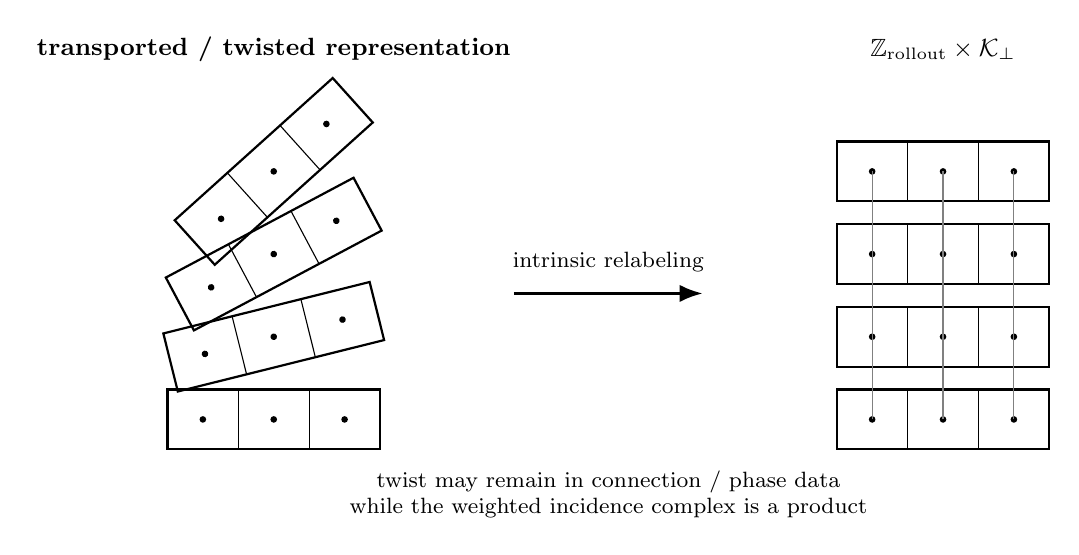
\begin{tikzpicture}[>=Latex,font=\small]
  \node[font=\small\bfseries] at (-4.25,4.70) {transported / twisted representation};
  \foreach \y/\ang in {0/0,1.05/14,2.10/28,3.15/42}{
    \begin{scope}[shift={(-4.25,\y)},rotate=\ang]
      \draw[thick] (-1.35,-0.38)--(1.35,-0.38)--(1.35,0.38)--(-1.35,0.38)--cycle;
      \draw (-0.45,-0.38)--(-0.45,0.38);
      \draw (0.45,-0.38)--(0.45,0.38);
      \fill (-0.90,0) circle (1.2pt);
      \fill (0,0) circle (1.2pt);
      \fill (0.90,0) circle (1.2pt);
    \end{scope}
  }

  \draw[->,very thick] (-1.20,1.60)--(1.20,1.60)
     node[midway,above=4pt,font=\footnotesize] {intrinsic relabeling};

  \node[font=\small\bfseries] at (4.25,4.70) {$\Z_{\rm rollout}\times\cK_\perp$};
  \foreach \y in {0,1.05,2.10,3.15}{
    \begin{scope}[shift={(4.25,\y)}]
      \draw[thick] (-1.35,-0.38)--(1.35,-0.38)--(1.35,0.38)--(-1.35,0.38)--cycle;
      \draw (-0.45,-0.38)--(-0.45,0.38);
      \draw (0.45,-0.38)--(0.45,0.38);
      \fill (-0.90,0) circle (1.2pt);
      \fill (0,0) circle (1.2pt);
      \fill (0.90,0) circle (1.2pt);
    \end{scope}
  }
  \foreach \x in {3.35,4.25,5.15}{\draw[gray] (\x,0)--(\x,3.15);}

  \node[align=center,font=\footnotesize] at (0,-0.95)
     {twist may remain in connection / phase data\\while the weighted incidence complex is a product};
\end{tikzpicture}
\caption{Exact intrinsic untwisting of the homogeneous transported transverse complex. The product statement concerns the weighted incidence structure, not the elimination of helical chirality or connection data.}
\label{fig:untwist}
\end{figure*}

\section{Cubic volume growth}

For the exact bulk theorem, equip the longitudinal chain with unit vertex measure and edge length \(\ell_\parallel\) satisfying
\[
0<\ell_{\parallel,-}\le \ell_\parallel\le \ell_{\parallel,+}<\infty,
\]
and use the product measure
\begin{equation}
\mu=\mu_\parallel\otimes\mu_\perp.
\end{equation}
More generally, uniformly comparable longitudinal node measures and edge lengths change only the comparison constants below.

\begin{proposition}[Three-dimensional volume-growth class]
Suppose the infinite homogeneous transverse complex satisfies the uniform quadratic growth condition
\begin{equation}
\mu_\perp(B_\perp(x,\rho))
\asymp
(1+\rho)^2
\label{eq:quadraticplus}
\end{equation}
for all sufficiently large \(\rho\), uniformly in \(x\). Under the exact product structure in Eq.~\eqref{eq:product},
\begin{equation}
\boxed{
\mu(B_{\cX}(r))\asymp r^3,
\qquad d_f=3
}
\label{eq:df3}
\end{equation}
for sufficiently large \(r\).
\end{proposition}

\begin{proof}
First take unit longitudinal edge length. In the exact product metric, a ball admits the section decomposition
\begin{equation}
\mu(B_{\cX}((0,o),r))
=
\sum_{|m|\le r}
\mu_\perp
\left(
B_\perp(o,r-|m|)
\right),
\label{eq:ballslice}
\end{equation}
up to the harmless integer rounding appropriate to graph distance.

Using Eq.~\eqref{eq:quadraticplus},
\begin{equation}
\mu(B_{\cX}(r))
\asymp
\sum_{|m|\le r}
(1+r-|m|)^2.
\end{equation}
The comparison sum has cubic growth. In the idealized unit-counting case,
\begin{equation}
\sum_{|m|\le r}(r-|m|)^2
=
\frac{2r^3+r}{3},
\end{equation}
so adding the endpoint \(1+\rho\) correction does not alter the exponent.

If longitudinal and transverse edge lengths are only uniformly comparable to the unit product, there exist constants \(a,b>0\) such that a product ball of radius \(ar\) is contained in the intrinsic ball and the intrinsic ball is contained in a product ball of radius \(br\). The same cubic upper and lower bounds therefore follow. Uniformly comparable longitudinal vertex measures likewise change only multiplicative constants. Hence
\[
\mu(B_{\cX}(r))\asymp r^3.
\]

\end{proof}

No Euclidean sphere measure \(4\pi r^2\) has been inserted into this proof.

\subsection{What is and is not derived here}

The theorem proves
\[
d_f=1+d_\perp=3
\]
for a transverse relational complex with \(d_\perp=2\). It does not prove in this paper that the full rollout ensemble must uniquely realize \(d_\perp=2\).

The result should therefore be read as:

\begin{quote}
A two-dimensionally organized source-local rollout ensemble, extended by regular non-dilational longitudinal rollout, stably realizes three-dimensional global volume growth.
\end{quote}

The deeper origin of the effective two-dimensional transverse organization is a separate microscopic problem.

\section{Controlled perturbations beyond the exact product}

The exact transported-complex ground state is the principal model. A broader rollout bundle remains coarsely equivalent to the product only under global, depth-independent control.

Let each transverse section \(\cK_m\) be connected and carry its intrinsic path metric. Suppose there exist maps
\[
\phi_m:\cK_m\rightarrow\cK_\perp
\]
with quasi-isometry constants \((L,A)\), coarse-surjectivity radius \(R_0\), and coarse-inverse error bounded by a common constant, all independent of \(m\). Assume also that longitudinal edges have lengths in a fixed interval
\[
0<\ell_{\parallel,-}\le \ell_\parallel\le \ell_{\parallel,+}<\infty.
\]
Finally require a bounded transport defect
\begin{equation}
d_\perp\!\left(
\phi_{m+1}(T_mx),
\phi_m(x)
\right)
\le D
\label{eq:defect}
\end{equation}
with \(D\) independent of \(m\) and \(x\).

\begin{proposition}[Uniformly controlled global trivialization]
Under the uniform conditions above and bounded local geometry, the map
\begin{equation}
\Phi(m,x)
=
(m,\phi_m(x))
\end{equation}
is a quasi-isometry from the rollout graph bundle to
\[
\Z\times\cK_\perp.
\]
\end{proposition}

\begin{proof}[Proof sketch]
A horizontal edge maps to a product path of uniformly bounded length because all \(\phi_m\) share the same quasi-isometry constants. A longitudinal edge maps to a product displacement bounded uniformly by \(\ell_{\parallel,+}+D\) because of Eq.~\eqref{eq:defect}. Thus \(\Phi\) is coarsely Lipschitz with constants independent of rollout depth.

For the reverse comparison, choose coarse inverse representatives in each section with a depth-independent error bound. A horizontal product step lifts with uniformly bounded distortion by the common quasi-isometry constants. A vertical product step from \((m,y)\) to \((m+1,y)\) is lifted by choosing \(x_m\) near a coarse inverse of \(y\); Eq.~\eqref{eq:defect}, together with the quasi-isometry lower bound in the next section, controls the distance between \(T_mx_m\) and a chosen coarse inverse representative \(x_{m+1}\). Hence a vertical product step lifts to a rollout-bundle path of uniformly bounded length. Concatenating such lifts gives a coarse inverse and a global affine comparison of distances.
\end{proof}

The depth-independent defect bound is essential. It is not sufficient that each \(T_m\) separately have a bounded quasi-isometry constant: repeated stretching can accumulate without a uniformly controlled global trivialization.

This proposition is a coarse-geometric statement. It does not by itself transfer weighted heat-kernel estimates to a perturbed rollout model. Such analytic stability additionally requires uniform control of measures, conductances, jump rates, and the hypotheses used in the diffusion theorem below.

\section{Normal diffusion from analytic regularity}

Cubic volume growth alone does not determine the walk dimension. Diffusion and spectral observables are standard probes of effective dimension in discrete spacetime models, including causal-set approaches \cite{EichhornMizera2014}. We therefore specify the analytic model used for the infinite homogeneous bulk.

Let \(L_\perp\) be the generator of a continuous-time reversible nearest-neighbor random walk on the weighted transverse graph underlying \(\cK_\perp\). Assume uniformly bounded local geometry, uniformly elliptic conductances and jump rates, volume doubling, and a scale-invariant Poincar\'e inequality on all sufficiently large scales. In the standard graph setting these hypotheses support parabolic Harnack control and diffusive two-sided heat-kernel estimates in the appropriate space-time regime \cite{Delmotte1999,Grigoryan2009}.

For clarity, the proof below uses the following explicit two-regime bounds. Let
\[
r=d_\perp(x,y).
\]
In the diffusive regime \(t\ge t_0\vee c_0 r\), with a fixed microscopic time \(t_0>0\), assume
\begin{equation}
p_t^\perp(x,y)
\asymp
\frac{1}{\mu_\perp(B_\perp(x,\sqrt t))}
\exp\!\left(
-c\,\frac{r^2}{t}
\right),
\label{eq:gaussperp}
\end{equation}
with the usual two-sided interpretation using possibly different positive constants. In the short-time off-diagonal regime \(0<t<c_0r\), assume the standard bounded-jump large-deviation upper control
\begin{equation}
p_t^\perp(x,y)
\le
C
\exp\!\left[
-c_1 r\log\!\left(1+\frac{r}{t}\right)
\right].
\label{eq:shorttail}
\end{equation}
The precise constants are immaterial for the scaling argument.

With quadratic transverse volume growth, the diffusive estimate becomes
\begin{equation}
p_t^\perp(x,y)
\asymp
t^{-1}
\exp\!\left(
-c\,\frac{r^2}{t}
\right)
\qquad (t\ge t_0\vee c_0r).
\end{equation}

Take the longitudinal factor to be the analogous continuous-time local walk on \(\Z\). For the exact product generator
\begin{equation}
L_{\cX}
=
L_\parallel\otimes I
+
I\otimes L_\perp,
\label{eq:productgenerator}
\end{equation}
the heat kernel factorizes. In its diffusive regime one obtains
\begin{equation}
p_t^{\cX}(X,Y)
\asymp
t^{-3/2}
\exp\!\left(
-C\,\frac{d_{\cX}(X,Y)^2}{t}
\right),
\label{eq:gauss3d}
\end{equation}
again with two-sided constants, above the microscopic time scale, and only in the space-time region where the bounded-jump graph walk is diffusive.

Equation~\eqref{eq:gauss3d} exhibits the characteristic relation
\[
d_{\cX}(X,Y)\sim t^{1/2}
\]
for long-scale transport. Hence the walk dimension is
\begin{equation}
\boxed{d_w=2.}
\label{eq:dw2}
\end{equation}

This conclusion uses the off-diagonal diffusive scale, not only the diagonal return-probability exponent.

\section{Large-distance \(1/r\) Green scaling}

We now distinguish the infinite homogeneous bulk theorem from finite-source realizations.

Assume first that the exact product model and the analytic conditions above hold on all sufficiently large scales of an infinite graph. Since \(d_f=3>d_w=2\), the continuous-time walk is transient in this bulk model, and
\begin{equation}
G(X,Y)
=
\int_0^\infty p_t^{\cX}(X,Y)\,\dd t
\end{equation}
is finite for \(X\ne Y\).

Let
\[
r=d_{\cX}(X,Y)\gg1.
\]
Choose a fixed constant \(a>0\) large enough that the interval \(t\ge ar\) lies in the diffusive space-time regime. Split
\begin{equation}
\begin{aligned}
G(X,Y)
&=
\int_0^{ar}p_t(X,Y)\,\dd t
+
\int_{ar}^{\infty}p_t(X,Y)\,\dd t\\
&=
G_{\rm short}+G_{\rm diff}.
\end{aligned}
\label{eq:greensplit}
\end{equation}

\paragraph{Diffusive contribution.}
Using the Gaussian upper bound,
\begin{equation}
G_{\rm diff}
\lesssim
\int_{ar}^{\infty}
t^{-3/2}
\exp\!\left(-c\frac{r^2}{t}\right)\dd t
\lesssim
\frac{1}{r}.
\end{equation}
For the lower bound, restrict to a window
\[
t\in[r^2,2r^2].
\]
There the Gaussian lower estimate gives
\[
p_t(X,Y)\gtrsim r^{-3},
\]
while the integration interval has length of order \(r^2\). Therefore
\begin{equation}
G_{\rm diff}\gtrsim \frac{1}{r}.
\end{equation}

\paragraph{Short-time and transition contribution.}
Write the product distance as \(r\asymp r_\parallel+r_\perp\). At least one factor distance is therefore bounded below by a fixed multiple of \(r\). For sufficiently short times, apply the bounded-jump large-deviation estimate to that factor and bound the other heat kernel by a uniform constant. In the remaining interval up to the fixed cutoff \(ar\), use the Gaussian upper bound once that factor has entered its diffusive regime. Consequently, for every fixed admissible \(a\) there are constants \(C_a,c_a>0\), independent of \(r,X,Y\), such that
\begin{equation}
p_t^{\cX}(X,Y)
\le
C_a e^{-c_a r},
\qquad 0<t\le ar,
\end{equation}
for all sufficiently large \(r\). Hence
\begin{equation}
G_{\rm short}
\le
C_a ar e^{-c_a r}
=
o(r^{-1}).
\end{equation}

Combining the two regimes gives the large-distance bulk law
\begin{equation}
\boxed{
G(X,Y)
\asymp
\frac{1}{d_{\cX}(X,Y)}
\qquad
\text{as }d_{\cX}(X,Y)\rightarrow\infty.
}
\label{eq:green}
\end{equation}

The symbol \(\asymp\) is intentional: the construction establishes a two-sided \(1/r\) scale, not an exact universal coefficient.

\subsection{Finite source and finite-age realizations}

Equation~\eqref{eq:green} is an infinite homogeneous bulk result. A finite-age source-local rollout universe may have a core, a finite rollout front, or other boundaries. Such boundaries can modify the global Green function even when local volume growth remains cubic.

The physically relevant expectation is therefore an intermediate-scale bulk regime,
\begin{equation}
\ell_{\rm micro}
\ll
r
\ll
L_{\rm boundary},
\end{equation}
in which the infinite-model scaling can be approximated before boundary effects dominate. Establishing the Green function of a specific finite rollout geometry requires its actual boundary conditions and is not done here.

\section{Hydrogen as a low-energy consistency check}

The microscopic volume-growth proof above does not use the hydrogen spectrum. Hydrogen is retained because its gross scaling provides a useful low-energy check on the same radial exponent.

Assume an effective attractive interaction
\begin{equation}
U(r)=-\frac{\kappa}{r^s},
\qquad \kappa>0,
\end{equation}
and a semiclassical characteristic action relation
\begin{equation}
J_n=nJ_0.
\end{equation}
With effective reduced inertial parameter \(\mu\),
\begin{equation}
E_n(r)
=
\frac{n^2J_0^2}{2\mu r^2}
-\frac{\kappa}{r^s}.
\end{equation}
Stationarity gives
\begin{equation}
r_n^{2-s}
=
\frac{n^2J_0^2}{\mu s\kappa},
\end{equation}
and stable negative-energy minima require
\[
0<s<2.
\]
The binding scale obeys
\begin{equation}
|E_n|
\propto
n^{-2s/(2-s)}.
\end{equation}
The hydrogenic gross law
\[
|E_n|\propto n^{-2}
\]
selects
\[
s=1.
\]

Thus a \(1/r\) effective attractive interaction reproduces the gross \(1/n^2\) scaling in this restricted semiclassical model. The statement made here is deliberately limited:

\begin{quote}
Hydrogenic gross scaling is a low-energy consistency check not used in the geometric and Green-kernel proofs above.
\end{quote}

The paper does not derive \(J_0=\hbar\), the physical electromagnetic coupling, fine structure, Lamb shifts, hyperfine effects, or the full hydrogen spectrum.

\section{Canonical product cells and common Hodge support}

Because the microscopic starting object is a transverse cell complex rather than only a graph, local two-cells do not have to be inferred from graph cycles after the fact.

Let \(I_m\) be the rollout interval joining section \(m\) to \(m+1\). The prismal construction gives:
\[
\text{vertex}\times I_m
\quad\rightarrow\quad
\text{longitudinal edge},
\]
\[
\text{transverse edge}\times I_m
\quad\rightarrow\quad
\text{mixed two-cell},
\]
and
\[
\text{transverse face}\times I_m
\quad\rightarrow\quad
\text{three-cell}.
\]

\begin{figure*}[t]
\centering
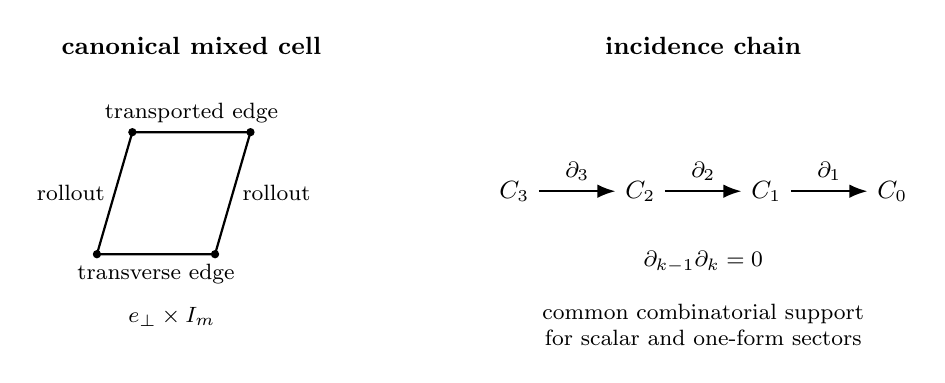
\begin{tikzpicture}[>=Latex,font=\small]
  \node[font=\small\bfseries] at (-3.2,3.1) {canonical mixed cell};
  \coordinate (a) at (-4.4,0.45);
  \coordinate (b) at (-2.9,0.45);
  \coordinate (c) at (-2.45,2.0);
  \coordinate (d) at (-3.95,2.0);
  \draw[thick] (a)--(b)--(c)--(d)--cycle;
  \fill (a) circle (1.5pt); \fill (b) circle (1.5pt);
  \fill (c) circle (1.5pt); \fill (d) circle (1.5pt);
  \node[below,font=\footnotesize] at ($(a)!0.5!(b)$) {transverse edge};
  \node[right,font=\footnotesize] at ($(b)!0.5!(c)$) {rollout};
  \node[above,font=\footnotesize] at ($(c)!0.5!(d)$) {transported edge};
  \node[left,font=\footnotesize] at ($(d)!0.5!(a)$) {rollout};
  \node[font=\footnotesize] at (-3.45,-0.35) {$e_\perp\times I_m$};

  \node[font=\small\bfseries] at (3.3,3.1) {incidence chain};
  \node (C3) at (0.9,1.25) {$C_3$};
  \node (C2) at (2.5,1.25) {$C_2$};
  \node (C1) at (4.1,1.25) {$C_1$};
  \node (C0) at (5.7,1.25) {$C_0$};
  \draw[->,thick] (C3)-- node[above,font=\footnotesize] {$\partial_3$} (C2);
  \draw[->,thick] (C2)-- node[above,font=\footnotesize] {$\partial_2$} (C1);
  \draw[->,thick] (C1)-- node[above,font=\footnotesize] {$\partial_1$} (C0);
  \node[font=\footnotesize] at (3.3,0.35) {$\partial_{k-1}\partial_k=0$};
  \node[align=center,font=\footnotesize] at (3.3,-0.45)
    {common combinatorial support\\for scalar and one-form sectors};
\end{tikzpicture}
\caption{Once the transverse structure is specified as a cell complex, rollout admits a canonical prismal cell attachment. This supplies a common incidence complex; it does not by itself determine the physical Hodge weights or low-energy coefficients.}
\label{fig:cells}
\end{figure*}

Thus
\begin{equation}
C_3
\xrightarrow{\partial_3}
C_2
\xrightarrow{\partial_2}
C_1
\xrightarrow{\partial_1}
C_0,
\qquad
\partial_{k-1}\partial_k=0.
\end{equation}

With metric and measure weights, one may define
\begin{equation}
\Delta_0=d_0^\dagger d_0,
\end{equation}
and
\begin{equation}
\Delta_1=d_0d_0^\dagger+d_1^\dagger d_1.
\end{equation}

The result established here is a common combinatorial-geometric support for these operators. It does not prove that all physical scalar, static, and transverse coefficients are already fixed by one microscopic TEF weight assignment. Harmonic modes, anisotropy, and normalization remain separate questions.

\section{Transverse-frame covariance and relational gluing}

The local transverse basis is not unique. Under a passive rotation by \(\chi\),
\begin{equation}
\begin{pmatrix}
\mathbf e_1'\\
\mathbf e_2'
\end{pmatrix}
=
\begin{pmatrix}
\cos\chi&\sin\chi\\
-\sin\chi&\cos\chi
\end{pmatrix}
\begin{pmatrix}
\mathbf e_1\\
\mathbf e_2
\end{pmatrix}.
\end{equation}
For a fixed transverse vector with complex component
\[
Z=X_1+iX_2,
\]
one has
\[
Z'=e^{-i\chi}Z.
\]
Thus the local transverse-frame group is
\begin{equation}
\boxed{\SO(2)\cong\U(1).}
\end{equation}

If transverse states at neighboring rollout locations must be compared, a link transport
\begin{equation}
U_{ij}=e^{-ia_{ij}}\in\U(1)
\end{equation}
may be used, transforming as
\begin{equation}
U_{ij}\rightarrow e^{-i\chi_i}U_{ij}e^{i\chi_j}.
\end{equation}

The canonical mixed two-cells constructed in the previous section provide local loops on which holonomy may be defined:
\begin{equation}
W_p
=
\prod_{\ell\in\partial p}U_\ell
=
e^{-i\Phi_p}.
\end{equation}

This identifies a natural place for the Abelian gluing structure developed in TEF. It does not establish that the physical electromagnetic field has already been derived. Whether lateral gluing is a genuine dynamical variable, how matter excitations source it, and how the observed coupling normalization emerges remain open.

\section{Discussion}

\subsection{What the construction establishes about the TEF spacetime view}

The main mathematical chain is now:

\conceptbox{source-local rollout ensemble $+$ effective quadratic-growth transverse relational complex $+$ regular screw-isometric longitudinal continuation}
\[
\Downarrow
\]
\[
\boxed{
\cK\cong\Z_{\rm rollout}\times\cK_\perp
\Longrightarrow
d_f=3
}
\]
and, under the stated analytic regularity,
\[
\boxed{
d_w=2
\Longrightarrow
G(r)\asymp 1/r.
}
\]

This is a forward construction rather than an inverse fit to the hydrogen spectrum, but it does not claim that one primitive helix uniquely forces three-dimensional space. The remaining structural question is why the complete rollout ensemble realizes a transverse relational complex in the quadratic-growth class; here that property is a TEF postulate whose consequences are tested.

\subsection{Why the ensemble matters more than one helix}

A single curve remains one-dimensional despite having a two-dimensional normal plane. TEF therefore assigns spatial significance to the full rollout ensemble, not to an isolated helix plus an abstract frame. The labels \(\alpha\in A_S\) identify neighboring trajectories; future microscopic work should derive their topology, metric, measure, and effective dimension from line-to-line relations. The same neighborhood structure is also required if excitations are collective modes of several rollout lines.

\subsection{Gauge-covariant multi-line phase coherence as the candidate excitation mechanism}

TEF treats an excitation as a possible phase-coherent collective mode of neighboring rollout trajectories. Related coherence-based transport ideas exist in recent relational frameworks \cite{Arneth2026PreEinsteinian,Arneth2026Twisted}; here the carrier is specifically the source-local helical rollout ensemble. If the line phases are compared using the same local transverse-frame convention as the \(\U(1)\)-type transport discussed above, a bare phase difference is not a physical observable: different lines may use different local frames.

Let
\[
\psi_\alpha=e^{i\phi_\alpha}
\]
denote a unit-modulus phase variable on rollout line \(\gamma_\alpha\). For relationally neighboring lines \(\alpha\) and \(\beta\), let
\[
U_{\alpha\beta}=e^{-ia_{\alpha\beta}}
\]
be the transverse transport from the \(\beta\)-fiber to the \(\alpha\)-fiber, with
\[
U_{\alpha\beta}
\rightarrow
e^{-i\chi_\alpha}
U_{\alpha\beta}
e^{i\chi_\beta},
\qquad
\psi_\alpha\rightarrow e^{-i\chi_\alpha}\psi_\alpha.
\]
Then
\begin{equation}
\psi_\alpha^*
U_{\alpha\beta}
\psi_\beta
\end{equation}
is invariant under independent local frame changes. Its phase defines the covariant relative phase
\begin{equation}
\Delta^{\rm cov}\phi_{\alpha\beta}
=
\phi_\beta-\phi_\alpha-a_{\alpha\beta}
\pmod{2\pi}.
\label{eq:covphase}
\end{equation}

A candidate local phase-locking condition is therefore
\begin{equation}
\boxed{
\Delta^{\rm cov}\phi_{\alpha\beta}
\approx
0
\quad (\mathrm{mod}\ 2\pi)
}
\label{eq:phaselock}
\end{equation}
over a connected cluster of neighboring rollout lines.

For a connected cluster \(C\) containing at least one edge, choose positive weights \(w_{\alpha\beta}>0\). A simple gauge-invariant coherence diagnostic is
\begin{equation}
\begin{aligned}
\mathcal C_C
&=
\frac{1}{\mathcal W_C}
\sum_{\langle\alpha\beta\rangle\subset C}
w_{\alpha\beta}
\cos\!\left(
\Delta^{\rm cov}\phi_{\alpha\beta}
\right),\\
\mathcal W_C
&=
\sum_{\langle\alpha\beta\rangle\subset C}w_{\alpha\beta}>0.
\end{aligned}
\label{eq:coherence}
\end{equation}
Values \(\mathcal C_C\) near unity indicate strong local covariant phase alignment. Exact locking on every edge of a closed loop is possible only when the corresponding loop holonomy is trivial: summing Eq.~\eqref{eq:covphase} around the loop cancels the vertex phases and leaves the connection holonomy. Nontrivial holonomy therefore produces phase-locking frustration, a feature to be addressed by a future excitation dynamics.

Equation~\eqref{eq:coherence} is only a candidate coherence diagnostic. A large value does not by itself prove localization, finite energy, dynamical stability, or a particle state. Those require an explicit excitation action and stability analysis.

One may alternatively parallel-transport all phases to a common reference fiber and form a collective order parameter. In a non-flat connection that construction is path dependent, so the required paths and holonomy must be specified. The edge-local diagnostic in Eq.~\eqref{eq:coherence} avoids hiding that issue.

These equations record the intended TEF ontology and a gauge-consistent target for later excitation dynamics; they are not used in the spacetime-growth proof.

\subsection{Source-local rollout cosmogenesis: the TEF ``Big-Bang'' analogy}

The same spacetime postulate suggests a source-local cosmogenesis. For a closed matter source \(S\),
\[
S\longrightarrow \cU_S
\]
represents a continuing realization of spatial relations. In this sense the process resembles a continuous ``TEF Big Bang'': the source does not first enter a supplied spatial world, but continually realizes additional rollout depth and relational structure. Unlike a conventional global Big-Bang description, the primitive object is source-local and the process is not assumed to be a single historical explosion.

A future finite-age realization might schematically be written as
\begin{equation}
\cU_S(t)
\sim
\{0,\ldots,M_S(t)\}\times\cK_{\perp,S}
\end{equation}
only as a bookkeeping picture, where \(M_S(t)\) denotes a rollout front measured in spatial depth. This expression is not part of the infinite-bulk theorem and no evolution law for \(M_S(t)\) is derived here.

No Friedmann law, Hubble relation, primordial history, or rollout-front dynamics is derived here. ``TEF Big Bang'' is therefore an interpretation of the spacetime ontology and a target for a future finite-front model, not a completed cosmological theory.

The central future question is how many source-local rollout universes
\[
\cU_{S_1},\cU_{S_2},\ldots
\]
produce one mutually accessible effective world. That requires a composition rule---through compatibility, overlap, gluing, rerouting, or another relational mechanism---rather than the assumption of a public background from the start.

\subsection{No automatic observable preferred frame}

A source-local ontology does not by itself imply an observable absolute rest frame. Recovering local relativistic symmetry is a strong consistency condition: if the construction necessarily produced a preferred inertial frame where none is observed, the postulates would require revision.

\begin{table*}[!t]
\centering
\small
\begin{tabular}{p{0.31\textwidth}p{0.61\textwidth}}
\toprule
\textbf{Item} & \textbf{Status in this paper}\\
\midrule
Closed matter as rollout source & TEF working postulate\\
Helical rollout ensemble & TEF working postulate\\
Effective transverse quadratic growth & Structural postulate; deeper origin unresolved\\
Screw-isometric homogeneous continuation & TEF ground-state postulate motivated by helix symmetry\\
Exact product after untwisting & Derived\\
\(d_f=3\) & Derived within stated postulates\\
Gaussian long-scale transport & Obtained under explicit graph-analytic regularity in the diffusive regime\\
\(d_w=2\) & Derived under those conditions\\
Large-distance \(G(r)\asymp1/r\) & Derived for the infinite homogeneous bulk using diffusive and short-time off-diagonal bounds\\
Hydrogenic \(1/n^2\) compatibility & Conditional low-energy check\\
Multi-line coherent excitation & TEF working postulate / future dynamics\\
Full electromagnetism and charge normalization & Not derived\\
\(J_0=\hbar\) & Not derived\\
Quantitative cosmology & Not derived\\
\bottomrule
\end{tabular}
\caption{Status of the principal TEF assumptions and results used in this paper.}
\label{tab:status}
\end{table*}

\subsection{Relation to the helix parameter \(q\)}

Dimensional growth and helix shape play different roles. The exponent \(d_f=3\) follows from the effective \(2+1\) relational organization and non-dilational continuation, while \(q\) may enter chirality, frame rotation, holonomy, operator weights, or dimensionless interaction data. Thus dimension can remain robust while coupling structure is sensitive to helix shape, consistent with earlier TEF work \cite{WuHelix2026,WuAlpha2026}.

\section{Falsifiability and current status}

The construction is hypothesis driven. Its postulates remain viable only while their consequences stay compatible with observation and later microscopic work reduces rather than proliferates assumptions. For a compact summary of the current status, see Table~\ref{tab:status}.


\section{Conclusion}

This paper gives a conditional mathematical realization of the TEF view that closed matter continuously realizes source-local spacetime relations. The working microscopic object is an ensemble of helical rollout trajectories with an effective transverse relational complex. In a homogeneous ground state, regular non-dilational transport carries that complex through spatial rollout depth.

If the transverse complex has quadratic growth and is transported by exact cell-complex isomorphisms, intrinsic untwisting yields
\[
\boxed{
\cK\cong\Z_{\rm rollout}\times\cK_\perp
}
\]
and hence
\[
\boxed{d_f=3.}
\]
Under the stated long-scale graph-analytic conditions, transport is normally diffusive,
\[
\boxed{d_w=2,}
\]
and the infinite homogeneous bulk has
\[
\boxed{
G(x,y)\asymp d(x,y)^{-1}
}
\]
at large separation. A finite-age source may reproduce this only over an intermediate bulk regime because its global Green function depends on the core, rollout front, and boundary conditions.

The construction also provides canonical product cells for a common incidence complex and a gauge-covariant language for multi-line coherence. It does not derive the transverse quadratic-growth class itself, a complete excitation dynamics, interaction normalization, or quantitative cosmology. Those are the next microscopic problems.

The resulting spacetime picture is nevertheless concrete: matter does not merely occupy a supplied spatial arena; each closed source realizes a source-local rollout universe. The ``TEF Big Bang'' is the corresponding interpretive statement---continuous source-local cosmogenesis rather than a theorem of cosmological expansion. A complete TEF spacetime theory must ultimately explain how many such source-local rollout structures compose into one mutually accessible effective world.

\begin{thebibliography}{99}

\bibitem{WuHelix2026}
X.~Wu,
\newblock \emph{A Helical Spacetime Ansatz Linking the Planck Scale and Electroweak Mixing},
\newblock Version 5.1, Zenodo (2026), DOI:
\href{https://doi.org/10.5281/zenodo.22101000}{10.5281/zenodo.22101000}.

\bibitem{WuAlpha2026}
X.~Wu,
\newblock \emph{From a Gravity-Calibrated Helix to a Conditional Fine-Structure Correspondence},
\newblock Version 4.7, Zenodo (2026), DOI:
\href{https://doi.org/10.5281/zenodo.22117153}{10.5281/zenodo.22117153}.

\bibitem{WuFramework2026}
X.~Wu,
\newblock \emph{The Emergent Frame: A Minimal Framework for Spacetime Rollout, Interaction, and Excitation},
\newblock Version 2.5, Zenodo (2026), DOI:
\href{https://doi.org/10.5281/zenodo.22723329}{10.5281/zenodo.22723329}.


\bibitem{Konopka2008}
T.~Konopka, F.~Markopoulou, and S.~Severini,
\newblock Quantum Graphity: a model of emergent locality,
\newblock \emph{Physical Review D} \textbf{77}, 104029 (2008),
\newblock arXiv:0801.0861 [hep-th],
DOI: \href{https://doi.org/10.1103/PhysRevD.77.104029}{10.1103/PhysRevD.77.104029}.

\bibitem{Oriti2007}
D.~Oriti,
\newblock Group field theory as the microscopic description of the quantum spacetime fluid: a new perspective on the continuum in quantum gravity,
\newblock arXiv:0710.3276 [gr-qc] (2007).

\bibitem{EichhornMizera2014}
A.~Eichhorn and S.~Mizera,
\newblock Spectral dimension in causal set quantum gravity,
\newblock \emph{Classical and Quantum Gravity} \textbf{31}, 125007 (2014),
\newblock arXiv:1311.2530 [gr-qc],
DOI: \href{https://doi.org/10.1088/0264-9381/31/12/125007}{10.1088/0264-9381/31/12/125007}.

\bibitem{Arneth2026PreEinsteinian}
B.~Arneth,
\newblock \emph{Pre-Einsteinian Coherent Relational Dynamics: A Pre-Geometric Framework for the Emergence of Quantum Theory, Gauge Structure, Probability, Matter, Spacetime, Gravitation, and Physical Constants from Stability-Selected Transport Organization},
\newblock Zenodo (2026),
DOI: \href{https://doi.org/10.5281/zenodo.20347721}{10.5281/zenodo.20347721}.

\bibitem{Arneth2026Twisted}
B.~Arneth,
\newblock \emph{Twisted Coherence Dirac Geometry and Spectral Emergence of Gauge--Matter Structure},
\newblock Zenodo (2026),
DOI: \href{https://doi.org/10.5281/zenodo.20413295}{10.5281/zenodo.20413295}.

\bibitem{Delmotte1999}
T.~Delmotte,
\newblock Parabolic Harnack inequality and estimates of Markov chains on graphs,
\newblock \emph{Revista Matem\'atica Iberoamericana} \textbf{15} (1999), 181--232.

\bibitem{Grigoryan2009}
A.~Grigor'yan,
\newblock \emph{Heat Kernel and Analysis on Manifolds},
\newblock AMS/IP Studies in Advanced Mathematics 47 (2009).


\end{thebibliography}

\end{document}
